\documentclass[runningheads]{llncs}


\usepackage{tikz}
\usepackage{calc}
\usepackage{amsmath,amssymb}
\usetikzlibrary{automata}






\begin{document}

\title{On finiteness of structures produced deterministically by co-transcriptional folding}

\section{Infiniteness of delay-1, arity-2 unary deterministic oritatami system}

\begin{figure}
  \begin{center}
    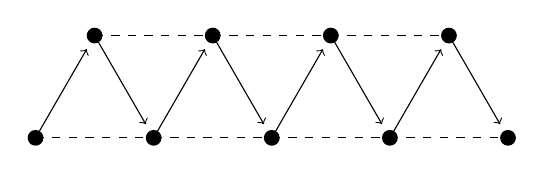
\begin{tikzpicture}
      \fill (0,0) circle[radius = 0.1];
      \fill (1.5,0) circle[radius = 0.1];
      \fill (3,0) circle[radius = 0.1];
      \fill (4.5,0) circle[radius = 0.1];
      \fill (6,0) circle[radius = 0.1];

      \draw[dashed] (0,0)--(1.5,0);
      \draw[dashed] (1.5,0)--(3,0);
      \draw[dashed] (3,0)--(4.5,0);
      \draw[dashed] (4.5,0)--(6,0);
      \draw[->] (0,0)--(60:1.3);
      \draw[->] (1.5,0)--++(60:1.3);
      \draw[->] (3,0)--++(60:1.3);
      \draw[->] (4.5,0)--++(60:1.3);
      
      \begin{scope}[shift=(60:1.5)]
        \fill (0,0) circle[radius = 0.1];
        \fill (1.5,0) circle[radius = 0.1];
        \fill (3,0) circle[radius = 0.1];
        \fill (4.5,0) circle[radius = 0.1];
        \draw[dashed] (0,0)--(1.5,0);
        \draw[dashed] (1.5,0)--(3,0);
        \draw[dashed] (3,0)--(4.5,0);
        \draw[->] (0,0)--(-60:1.3);
        \draw[->] (1.5,0)--++(-60:1.3);
        \draw[->] (3,0)--++(-60:1.3);
        \draw[->] (4.5,0)--++(-60:1.3);
      \end{scope}
      
    \end{tikzpicture}
    \caption{zig-zag conformation}
    \label{TTT_zigzag}
  \end{center}
\end{figure}

\subsection{Introduction}


In this section, we prove that unary oritatami system can form infinitely at delay 1 and arity 2 deterministically and moreover that the only infinite conformations which its oritatami system can yield is only the zig-zag conformation shown in Fig.\ref{TTT_zigzag}. 


Let $\Xi$ be a deterministic oritatami system of delay 1 and arity 2. Assume its seed $\sigma$ consists of $n$ beads.
%Let us denote its transcript by $w = w_1 w_2 w_3 \cdots$ for some $w_1,w_2,w_3 \in \Sigma = \{e\}$.
For $i \geq 0$ let $C_i$ be the unique elongation of $\sigma$ by $w[1..i]$ that is foldable by $\Xi$. Hence $C_0 = \sigma$.


Let us consider the stabilization of the $i$-th bead $a_i$ upon $C_{i-1}$. The bead cannot collaborate with any succeeding bead $w[i+1],w[i+2],\cdots$ at delay 1. There are just two ways to get stabilized at delay 1. One way is to be bound to another bead. The other way is through a $tunnel\ section$. A tunnel section consists of four beads that occupy four neighbors of a point (Fig.\ref{TTT_tunnel_intro}). Assume that four of the six neighbors of a point $p$ are occupied by beads $a_{j_1},a_{j_2},a_{j_3},a_{j_4}$ while the other two are free. We call such beads as $p$ $inside\ of\ a\ tunnel$ and such beads as $p^\prime$ $entrance\ of\ a\ tunnel$ without a case that $p^\prime$ is inside of a tunnel. If the beads $w[i-2]$ and $w[i-1]$ are stabilized respectively at one of the two free neighbors and at $p$ one after another, then the next bead $w[i]$ cannot help but be stabilized at the other free neighbor. In this way, $w[i]$ can get stabilized without being bound.



If a bead is stabilized through a tunnel section, then it can provide two binging capabilities and create tunnel sections.



\begin{figure}
  \begin{center}
    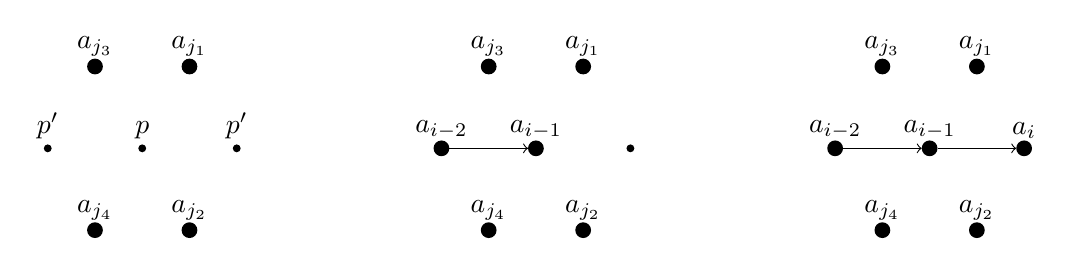
\begin{tikzpicture}
      \fill (0:0) circle [radius=0.05];
      \fill (0:1.2) circle [radius=0.05];
      \fill (180:1.2) circle [radius=0.05];
      \node[above] at (0:1.2) { $p^\prime$ };
      \node[above] at (0:0) { $p$ };
      \node[above] at (180:1.2) { $p^\prime$ };
      
      \fill (60 : 1.2) circle [radius=0.1];
      \fill (-60 : 1.2) circle [radius=0.1];
      \fill (120 : 1.2) circle [radius=0.1];
      \fill (-120 : 1.2) circle [radius=0.1];
      \node[above] at (60 :1.2) { $a_{j_1}$ };
      \node[above] at (-60 :1.2) { $a_{j_2}$ };
      \node[above] at (120 :1.2) { $a_{j_3}$ };
      \node[above] at (-120 :1.2) { $a_{j_4}$ };
      
      \begin{scope}[shift=(0:5)]
        \fill (0:0) circle [radius=0.1];
        \fill (0:1.2) circle [radius=0.05];
        \fill (180:1.2) circle [radius=0.1];
        \node[above] at (180:1.2) { $a_{i-2}$ };
        \node[above] at (0:0) { $a_{i-1}$ };
        \draw[->] (180:1.1) -- (180:0.1);
        
        \fill (60 : 1.2) circle [radius=0.1];
        \fill (-60 : 1.2) circle [radius=0.1];
        \fill (120 : 1.2) circle [radius=0.1];
        \fill (-120 : 1.2) circle [radius=0.1];
        \node[above] at (60 :1.2) { $a_{j_1}$ };
        \node[above] at (-60 :1.2) { $a_{j_2}$ };
        \node[above] at (120 :1.2) { $a_{j_3}$ };
        \node[above] at (-120 :1.2) { $a_{j_4}$ };
      \end{scope}
      \begin{scope}[shift=(0:10)]
        \fill (0:0) circle [radius=0.1];
        \fill (0:1.2) circle [radius=0.1];
        \fill (180:1.2) circle [radius=0.1];
        \node[above] at (180:1.2) { $a_{i-2}$ };
        \node[above] at (0:0) { $a_{i-1}$ };
        \node[above] at (0:1.2) { $a_i$ };
        \draw[->] (180:1.1) -- (180:0.1);
        \draw[->] (0:0.1) -- (0:1.1);
        
        \fill (60 : 1.2) circle [radius=0.1];
        \fill (-60 : 1.2) circle [radius=0.1];
        \fill (120 : 1.2) circle [radius=0.1];
        \fill (-120 : 1.2) circle [radius=0.1];
        \node[above] at (60 :1.2) { $a_{j_1}$ };
        \node[above] at (-60 :1.2) { $a_{j_2}$ };
        \node[above] at (120 :1.2) { $a_{j_3}$ };
        \node[above] at (-120 :1.2) { $a_{j_4}$ };
      \end{scope}
    \end{tikzpicture} 
    \caption{Through a tunnel section}
    \label{TTT_tunnel_intro}
  \end{center}
\end{figure}




\begin{theorem}[Tunnel Troll Theorem]
  Let $\Xi$ be an unary oritatami system of delay 1 and arity 2. If a bead is stabilized through a tunnel section, then it consume some binging capabilities.
\end{theorem}

\subsection{Proof of Tunnel Troll Theorem}
Assume $\Xi$ is deterministic. Let us represent its transcript $w$ as $w = w_1 w_2 w_3 \cdots$ for beads $w_1 , w_2 , w_3 , \cdots \in \Sigma = \{e\}$. Each of these beads is stabilized either by being bound or through a tunnel section (or by both). How they are stabilized can be described by a binary sequence $S$ of $b$'s (bound) and $t$'s (tunnel section); priority is given to $t$, that is, $S[i] = t$ if the $i$-th bead $w_i$ is stabilized not only by being bound but also through a tunnel section. 
On the other hand, each of beads are bound either inside of tunnel or outside (Fig. \ref{TTT_position1}). If a bead is stabilized at inside of tunnel, then its successor is already decided the position either inside of a tunnel or outside. Moreover, If a bead is stabilized at outside of a tunnel, then its position is an entrance of a tunnel or otherwise.


Tunnel sections have three possible shape with considering symmetry such as acute turn, straight and obtuse turn (Figure \ref{TTT_tunnel}). Let us focus entrances of a tunnel such as $p^\prime$, then Entrances have two possible shape (Figure \ref{TTT_enterpoint}).


Let us consider tunnel sections only tunnel A and B. See Fig. \ref{TTT_position2}. From appendix (Entrance of Tunnel A, B and Exit of Tunnel), we add maximum number which each transitions provide binding capabilities for each edge where $a$ is number of consuming binding capabilities when the bead is stabilized at position of $successer\ in\ outside$.


Next, we consider on tunnel C section. If $w[i]$ is stabilized by tunnel C and $S[i+1]$ is $t$, then $w[i+1]$ is stabilized by tunnel A or B because if $w[i+1]$ is stabilized by tunnel C, then $C_{i+1}$ is a terminal. Hence, tunnel C section is devided cases sush as Figure \ref{TTT_tunnelC_graph}. Cases of $S[i...] = bt^l (l \geq 2)$ are already considered (Upper). According to appendix (Tunnel C), cases of $S[i..i+2] = btb$ also consume some binding capabilities (Lower).


Thus, if a bead is stabilized through a tunnel section, then it consume some binging capabilities.



\begin{figure}
  \begin{center}
    \begin{tabular}{ccc}
      
      \begin{minipage}{0.3\hsize}
        \begin{tikzpicture}
          \begin{scope}[xshift=2cm, yshift=2cm]
            \fill(0,0) circle [radius=0.05];
            \node[above] at (180:1.2) {$p^\prime$};
            \node[above] at (0:1.2) {$p^\prime$};

            \foreach \theta in {0,180}{
              \fill[transform canvas={shift=(\theta:1.2)}](0,0) circle [radius=0.05];
            }
            
            \foreach \theta in {60,-60,120,-120}{
              \draw[transform canvas={shift=(\theta:1.2)}](-0.1,-0.1)--(0.1,0.1);
              \draw[transform canvas={shift=(\theta:1.2)}](0.1,-0.1)--(-0.1,0.1);
            }
          \end{scope}

          \node at (2,0) {Tunnel A};
        \end{tikzpicture}
      \end{minipage}

      \begin{minipage}{0.3\hsize}
        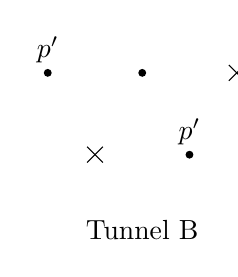
\begin{tikzpicture}

          \begin{scope}[xshift=2cm, yshift=2cm]
            \fill(0,0) circle [radius=0.05];
            \node[above] at (180:1.2) {$p^\prime$};
            \node[above] at (-60:1.2) {$p^\prime$};

            \foreach \theta in {-60,180}{
              \fill[transform canvas={shift=(\theta:1.2)}](0,0) circle [radius=0.05];
            }
            
            \foreach \theta in {0,60,120,-120}{
              \draw[transform canvas={shift=(\theta:1.2)}](-0.1,-0.1)--(0.1,0.1);
              \draw[transform canvas={shift=(\theta:1.2)}](0.1,-0.1)--(-0.1,0.1);
            }
          \end{scope}

          \node at (2,0) {Tunnel B};
        \end{tikzpicture}
      \end{minipage}

      \begin{minipage}{0.3\hsize}
        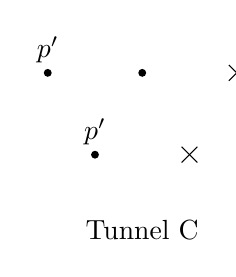
\begin{tikzpicture}

          \begin{scope}[xshift=2cm, yshift=2cm]
            \fill(0,0) circle [radius=0.05];
            \node[above] at (180:1.2) {$p^\prime$};
            \node[above] at (-1200:1.2) {$p^\prime$};

            \foreach \theta in {-120,180}{
              \fill[transform canvas={shift=(\theta:1.2)}](0,0) circle [radius=0.05];
            }
            
            \foreach \theta in {0,60,-60,120}{
              \draw[transform canvas={shift=(\theta:1.2)}](-0.1,-0.1)--(0.1,0.1);
              \draw[transform canvas={shift=(\theta:1.2)}](0.1,-0.1)--(-0.1,0.1);
            }
          \end{scope}

          \node at (2,0) {Tunnel C};
        \end{tikzpicture}
      \end{minipage}
      
    \end{tabular}
    \caption{All possible tunnel sections}
    \label{TTT_tunnel}
  \end{center}
\end{figure}

\begin{figure}
  \begin{center}
    \begin{tabular}{lr}
      
      \begin{minipage}{0.2\hsize}
        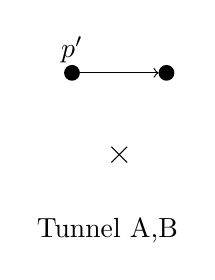
\begin{tikzpicture}

          \begin{scope}[xshift=1cm, yshift=2cm]
            \fill(0,0) circle [radius=0.1];
            \node[above] at (180:1.2) {$p^\prime$};
            
            \fill[transform canvas={shift=(180:1.2)}](0,0) circle [radius=0.1];
            
            
            \foreach \theta in {120,-120}{
              \draw[transform canvas={shift=(\theta:1.2)}](-0.1,-0.1)--(0.1,0.1);
              \draw[transform canvas={shift=(\theta:1.2)}](0.1,-0.1)--(-0.1,0.1);
            }

            \draw[->] (-1.1,0) -- (-0.1,0);
          \end{scope}

          \node at (0.25,0) {Tunnel A,B};
        \end{tikzpicture}
      \end{minipage}

      \begin{minipage}{0.2\hsize}
        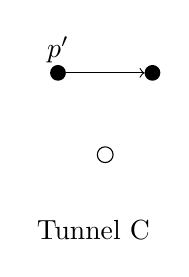
\begin{tikzpicture}

          \begin{scope}[xshift=1cm, yshift=2cm]
            \fill(0,0) circle [radius=0.1];
            \node[above] at (180:1.2) {$p^\prime$};

            \draw[transform canvas={shift=(-120:1.2)}](0,0) circle [radius=0.1];
            \fill[transform canvas={shift=(180:1.2)}](0,0) circle [radius=0.1];
            
            
            \foreach \theta in {120}{
              \draw[transform canvas={shift=(\theta:1.2)}](-0.1,-0.1)--(0.1,0.1);
              \draw[transform canvas={shift=(\theta:1.2)}](0.1,-0.1)--(-0.1,0.1);
            }

            \draw[->] (-1.1,0) -- (-0.1,0);
          \end{scope}

          \node at (0.25,0) {Tunnel C};
        \end{tikzpicture}
      \end{minipage}

    \end{tabular}
    \caption{Entrance of a tunnel}
    \label{TTT_enterpoint}
  \end{center}
\end{figure}



\begin{figure}
  \begin{center}
    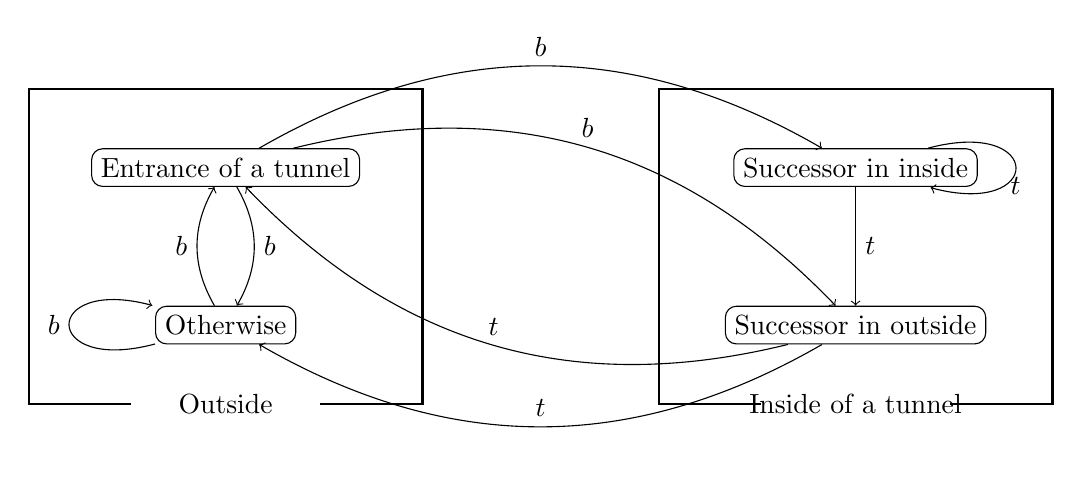
\begin{tikzpicture}
      \draw[thick]
      (1.3,1)--(0,1)--(0,5)--(5,5)--(5,1)--(3.7,1);
      \node at(2.5,1) {Outside};
      \node at (2.5,4) [rectangle, draw,rounded corners] (enter) {Entrance of a tunnel};
      \node at(2.5,2) [rectangle, draw, rounded corners] (outside) {Otherwise};

      
      
      \draw[thick]
      (9.3,1)--(8,1)--(8,5)--(13,5)--(13,1)--(11.7,1);
      \node at(10.5,1) {Inside of a tunnel};
      \node at(10.5,4) [rectangle, draw, rounded corners] (next-tunnel) {Successor in inside};
      \node at(10.5,2) [rectangle, draw, rounded corners] (next-outside) {Successor in outside};

      \draw[->]
      (outside) edge [bend left] node[left] {$b$} (enter)
                edge [loop left] node[left] {$b$} (outside)
      (enter)   edge [bend left] node[above] {$b$} (next-tunnel)
                edge [bend left] node[above] {$b$} (next-outside)
                edge [bend left] node[right] {$b$}  (outside)
      (next-tunnel) edge         node[right] {$t$} (next-outside)
                edge [loop right]node[below] {$t$}    (next-tunnel)
      (next-outside) edge[bend left] node[above] {$t$}  (outside)
                edge [bend left]     node[above] {$t$}(enter)
      ;
      
    \end{tikzpicture}
    \caption{Cases on position of a bead}
    \label{TTT_position1}
  \end{center}
\end{figure}

\begin{figure}
  \begin{center}
    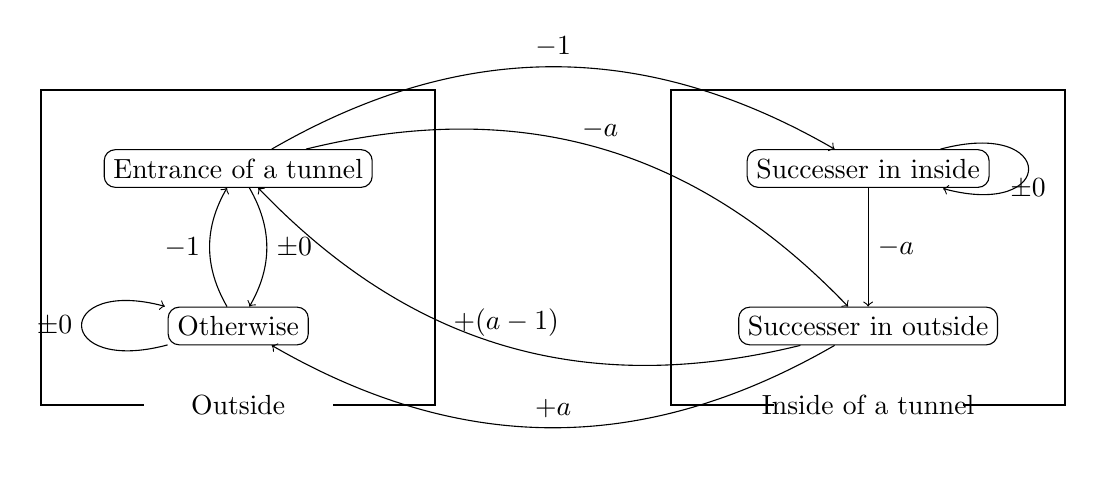
\begin{tikzpicture}
      \draw[thick]
      (1.3,1)--(0,1)--(0,5)--(5,5)--(5,1)--(3.7,1);
      \node at(2.5,1) {Outside};
      \node at (2.5,4) [rectangle, draw,rounded corners] (enter) {Entrance of a tunnel};
      \node at(2.5,2) [rectangle, draw, rounded corners] (outside) {Otherwise};

      
      
      \draw[thick]
      (9.3,1)--(8,1)--(8,5)--(13,5)--(13,1)--(11.7,1);
      \node at(10.5,1) {Inside of a tunnel};
      \node at(10.5,4) [rectangle, draw, rounded corners] (next-tunnel) {Successer in inside};
      \node at(10.5,2) [rectangle, draw, rounded corners] (next-outside) {Successer in outside};

      \draw[->]
      (outside) edge [bend left] node[left] {$-1$} (enter)
                edge [loop left] node[left] {$\pm 0$} (outside)
      (enter)   edge [bend left] node[above] {$-1$} (next-tunnel)
                edge [bend left] node[above] {$-a$} (next-outside)
                edge [bend left] node[right] {$\pm 0$}  (outside)
      (next-tunnel) edge         node[right] {$-a$} (next-outside)
                edge [loop right]node[below] {$\pm 0$}    (next-tunnel)
      (next-outside) edge[bend left] node[above] {$+a$}  (outside)
                edge [bend left]     node[above] {$+(a-1)$}(enter)
      ;
      
    \end{tikzpicture}
    \caption{Increment on Tunnel A,B}
    \label{TTT_position2}
  \end{center}
\end{figure}

\begin{figure}
  \begin{center}
    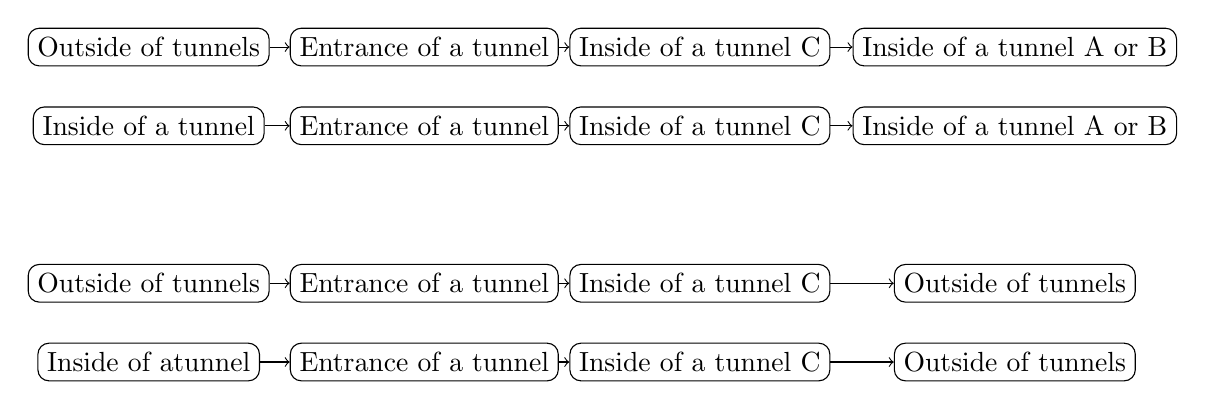
\begin{tikzpicture}
      \node at (0,4)   [rectangle, draw,rounded corners] (outside1) {Outside of tunnels};
      \node at (3.5,4) [rectangle, draw,rounded corners] (enter1)   {Entrance of a tunnel};
      \node at (7,4)   [rectangle, draw, rounded corners] (inside1) {Inside of a tunnel C};
      \node at (11,4)  [rectangle, draw, rounded corners] (exit1)   {Inside of a tunnel A or B};
      \draw[->] (outside1)--(enter1);
      \draw[->] (enter1)  --(inside1);
      \draw[->] (inside1) --(exit1);
      
      
      \node at (0,3)   [rectangle, draw,rounded corners] (outside2) {Inside of a tunnel};
      \node at (3.5,3) [rectangle, draw,rounded corners] (enter2)   {Entrance of a tunnel};
      \node at (7,3)   [rectangle, draw, rounded corners] (inside2) {Inside of a tunnel C};
      \node at (11,3)  [rectangle, draw, rounded corners] (exit2)   {Inside of a tunnel A or B};     
      \draw[->] (outside2)--(enter2);
      \draw[->] (enter2)  --(inside2);
      \draw[->] (inside2) --(exit2);

      \node at (0,1)   [rectangle, draw,rounded corners] (outside3) {Outside of tunnels};
      \node at (3.5,1) [rectangle, draw,rounded corners] (enter3)   {Entrance of a tunnel};
      \node at (7,1)   [rectangle, draw, rounded corners] (inside3) {Inside of a tunnel C};
      \node at (11,1)  [rectangle, draw, rounded corners] (exit3)   {Outside of tunnels};     
      \draw[->] (outside3)--(enter3);
      \draw[->] (enter3)  --(inside3);
      \draw[->] (inside3) --(exit3);

      \node at (0,0)   [rectangle, draw,rounded corners] (outside4) {Inside of atunnel};
      \node at (3.5,0) [rectangle, draw,rounded corners] (enter4)   {Entrance of a tunnel};
      \node at (7,0)   [rectangle, draw, rounded corners] (inside4) {Inside of a tunnel C};
      \node at (11,0)  [rectangle, draw, rounded corners] (exit4)   {Outside of tunnels};     
      \draw[->] (outside4)--(enter4);
      \draw[->] (enter4)  --(inside4);
      \draw[->] (inside4) --(exit4);
    \end{tikzpicture}
    \caption{Case of Tunnel C}
    \label{TTT_tunnelC_graph}
  \end{center}
\end{figure}


\subsection{Appendix of Tunnel Troll Theorem}
\subsubsection{Entrance of TunnelA,B}

Fig.\ref{TTT_tunnel_direction} exhibits all the three kinds of entrance of tunnel A, B.
Any cases in $\delta = 1, \alpha = 2$ consume some binding capabilities into the follows.


\begin{itemize}
\item{Case of $t_0$}\\
  Let us consider points of $c,d$ either occupied or not. A point $c$ or $d$ is free because if both of them are occupied, $p^\prime$ is inside of tunnel. If $c$ is free, then $p^\prime$ has to be bound to a bead except $A$ due to deterministically stabilize. In this situation, at least three neighbors of A are free that is at most three neighbors of A are occupied. A leave at least one binging capability because beads of beighbors are predecessor and successor in addition A is able to consume itself binging capabilities only one-time. Hence, $p^\prime$ must be bound to A. Thus, a case of $t_0$ consumes some binding capabilities.

\item{Case of $t_{\pm 60}$}\\
  In this case, a point $c$ or $d$ is free, too. If $c$ is free, $p^\prime$ has to be bound to A or B. If $c$ is occupied, then $d$ is free. This time, B has some binding capabilitie so $p^\prime$ has to be bound to B.
  

  In this situation, $p^\prime$ is able to supply a binding capability. if this capability is active, $p^\prime$ bind a bead into $c$ or $d$. However, B and P are exist in back bone. According to Jordan curve theorem, any successors of $p^\prime$ cannot reach a point $c$ or $d$ so this capability is inactive. Thus, a case of $t_{\pm 60}$ consumes some binding capabilities.

\item{Case of $t_{\pm 120}$}\\
  Binding capabilities that $p^\prime$ supply are inactive according to Jordan curve theorem on A and P. Moreover, $p^\prime$ has to be bound to one of $c$, $d$,$e$ in order to deterministically stabilize.
Thus, a case of $t_{\pm 120}$ consumes some binging capabilities.
  
\end{itemize}

\begin{figure}
  \begin{center}
    \begin{tabular}{ccc}
      
      \begin{minipage}{0.3\hsize}
        \begin{tikzpicture}

          \begin{scope}[xshift=2cm, yshift=2cm]
            \fill(0,0) circle [radius=0.1];
            \node[above] at (0,0) {$p^\prime$};

            \foreach \theta in {0}{
              \draw[transform canvas={shift=(\theta:1.2)}](0,0) circle [radius=0.1];
            }
            
            \foreach \theta in {60,-60,180}{
              \draw[transform canvas={shift=(\theta:1.2)}](-0.1,-0.1)--(0.1,0.1);
              \draw[transform canvas={shift=(\theta:1.2)}](0.1,-0.1)--(-0.1,0.1);
            }

            \foreach \theta in {120,-120}{
              \draw[transform canvas={shift=(\theta:1.2)}](-0.1,-0.1) rectangle (0.1,0.1);
            }

            \draw[->] (180:1.1)--(180:0.1);
            \draw[->] (0:0.1)--(0:1.1);

            \node[transform canvas={shift=(60:1.2)},right] {A};
            \node[transform canvas={shift=(-60:1.2)},right] {B};

            \node[transform canvas={shift=(120:1.2)},left] {c};
            \node[transform canvas={shift=(-120:1.2)},left] {d};
          \end{scope}

          \node at (2,-0.5) {$t_0$};
        \end{tikzpicture}
      \end{minipage}

      \begin{minipage}{0.3\hsize}
        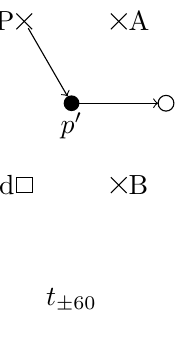
\begin{tikzpicture}

          \begin{scope}[xshift=2cm, yshift=2cm]
            \fill(0,0) circle [radius=0.1];
            \node[below] at (0,0) {$p^\prime$};

            \foreach \theta in {0}{
              \draw[transform canvas={shift=(\theta:1.2)}](0,0) circle [radius=0.1];
            }
            
            \foreach \theta in {60,-60,120}{
              \draw[transform canvas={shift=(\theta:1.2)}](-0.1,-0.1)--(0.1,0.1);
              \draw[transform canvas={shift=(\theta:1.2)}](0.1,-0.1)--(-0.1,0.1);
            }

            \foreach \theta in {180,-120}{
              \draw[transform canvas={shift=(\theta:1.2)}](-0.1,-0.1) rectangle (0.1,0.1);
            }
            
            \draw[->] (120:1.1)--(120:0.1);
            \draw[->] (0:0.1)--(0:1.1);

            \node[transform canvas={shift=(60:1.2)},right] {A};
            \node[transform canvas={shift=(-60:1.2)},right] {B};
            \node[transform canvas={shift=(120:1.2)},left] {P};

            \node[transform canvas={shift=(180:1.2)},left] {c};
            \node[transform canvas={shift=(-120:1.2)},left] {d};
          \end{scope}

          \node at (2,-0.5) {$t_{\pm 60}$};
        \end{tikzpicture}
      \end{minipage}

      \begin{minipage}{0.3\hsize}
        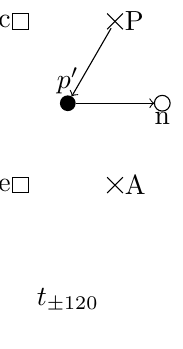
\begin{tikzpicture}

          \begin{scope}[xshift=2cm, yshift=2cm]
            \fill(0,0) circle [radius=0.1];
            \node[above] at (0,0) {$p^\prime$};

            \foreach \theta in {0}{
              \draw[transform canvas={shift=(\theta:1.2)}](0,0) circle [radius=0.1];
            }
            
            \foreach \theta in {60,-60}{
              \draw[transform canvas={shift=(\theta:1.2)}](-0.1,-0.1)--(0.1,0.1);
              \draw[transform canvas={shift=(\theta:1.2)}](0.1,-0.1)--(-0.1,0.1);
            }

            \foreach \theta in {180,-120,120}{
              \draw[transform canvas={shift=(\theta:1.2)}](-0.1,-0.1) rectangle (0.1,0.1);
            }
            
            \draw[->] (60:1.1)--(60:0.1);
            \draw[->] (0:0.1)--(0:1.1);

            \node[transform canvas={shift=(-60:1.2)},right] {A};
            \node[transform canvas={shift=(60:1.2)},right] {P};

            \node[transform canvas={shift=(120:1.2)},left] {c};
            \node[transform canvas={shift=(180:1.2)},left] {d};
            \node[transform canvas={shift=(-120:1.2)},left] {e};
            \node[transform canvas={shift=(0:1.2)},below] {n};
          \end{scope}

          \node at (2,-0.5) {$t_{\pm 120}$};
        \end{tikzpicture}
      \end{minipage}
      
    \end{tabular}
    \caption{Direction into a entrance}
    \label{TTT_tunnel_direction}
  \end{center}
\end{figure}


\subsubsection{Exit of Tunnel}


Fig.\ref{TTT_tunnel_exit} exhibits all the two kings of exit of tunnel. 
At least one of point $c$ or $d$ is free because if both of them are occupied, $p^\prime$ is inside of tunnel.

\paragraph{$\delta = 1, \alpha = 2$}
 Any cases of $\delta = 1, \alpha = 2$ supply at most $a$ binding capabilities into follows where $a$ is number of predecessor of $p^\prime$ consumes binging capabilities.

\begin{itemize}
\item{Case of $c$ and $d$ are free}\\
  This case can be regarded same situation as entrance. See Fig.\ref{TTT_tunnel_exit} (Left). Predecessor P has to be bound A and B because each of A and B leave binding capabilities. Hence, at least $a=2$. This time, $\alpha = 2$ that is this case supply at most only $a$ binding capabilities.
  
\item{Case of $c$ is occupied}\\
  See Fig.\ref{TTT_tunnel_exit} (Right). If $c$ is pccupied, then $d$ is free so that P has to be bound B. Hence, at least $a=1$. This case can supply two binding capabilities but $p^\prime$ can bind to only one of $e$ or $d$ because $e$ or $d$ will be occupied a successor of $p^\prime$. Therefore, this case supply at most only $a=1$ active binding capabiliry.
  
\end{itemize}

\paragraph{$\delta = 1, \alpha \geq 3$}
Any cases of $\delta = 1, \alpha \geq 3$ consume some binding capabilities into follows.

\begin{itemize}
\item{Case of $c$ and $d$ are free}\\
  In $\alpha \geq 3$, if three neighbors of a bead leave, then it can supply two binding capabilities. Therefore Predecessor P has to be bound A and B, and $p^\prime$, too. In this case, at least consumes four bindings and supplies at most two bindings. Thus, it consumes some binding capabilities, totally.
  
\item{Case of $c$ is occupied}\\
  In this case, B leave at least two bindings and A, $c$ also leave at least one binding. Therefore P has to be bound A and B, and $p^\prime$ also has to be bound B and $c$. In this case, at least consumes four bindings and supplies at most one binding. Thus, it consumes some binding capabiliries, totally.
\end{itemize}


\begin{figure}
  \centering
    \begin{tabular}{cc}
      
      \begin{minipage}{0.48\linewidth}
      \centering
        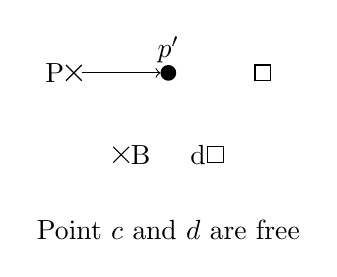
\begin{tikzpicture}

            \fill(0,0) circle [radius=0.1];
            \node[above] at (0,0) {$p^\prime$};

            
            \foreach \theta in {120,-120,180}{
              \draw[transform canvas={shift=(\theta:1.2)}](-0.1,-0.1)--(0.1,0.1);
              \draw[transform canvas={shift=(\theta:1.2)}](0.1,-0.1)--(-0.1,0.1);
            }

            \foreach \theta in {0,60,-60}{
              \draw[transform canvas={shift=(\theta:1.2)}](-0.1,-0.1) rectangle (0.1,0.1);
            }

            \draw[->] (180:1.1)--(180:0.1);

            \node[transform canvas={shift=(120:1.2)},right] {A};
            \node[transform canvas={shift=(-120:1.2)},right] {B};
            \node[transform canvas={shift=(180:1.2)},left] {P};

            \node[transform canvas={shift=(60:1.2)},left] {c};
            \node[transform canvas={shift=(-60:1.2)},left] {d};

          \node at (0,-2) {Point $c$ and $d$ are free};
        \end{tikzpicture}
      \end{minipage}

      \begin{minipage}{0.48\linewidth}
      \centering
        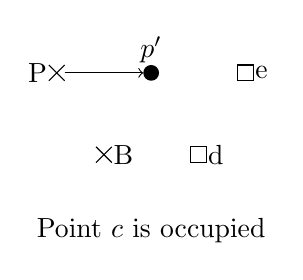
\begin{tikzpicture}

            \fill(0,0) circle [radius=0.1];
            \node[above] at (0,0) {$p^\prime$};
            
            \foreach \theta in {120,-120,180,60}{
              \draw[transform canvas={shift=(\theta:1.2)}](-0.1,-0.1)--(0.1,0.1);
              \draw[transform canvas={shift=(\theta:1.2)}](0.1,-0.1)--(-0.1,0.1);
            }

            \foreach \theta in {0,-60}{
              \draw[transform canvas={shift=(\theta:1.2)}](-0.1,-0.1) rectangle (0.1,0.1);
            }

            \draw[->] (180:1.1)--(180:0.1);

            \node[transform canvas={shift=(120:1.2)},right] {A};
            \node[transform canvas={shift=(-120:1.2)},right] {B};
            \node[transform canvas={shift=(180:1.2)},left] {P};

            \node[transform canvas={shift=(-60:1.2)},right] {d};
            \node[transform canvas={shift=(60:1.2)},right] {c};
            \node[transform canvas={shift=(0:1.2)},right] {e};

          
          \node at (0,-2) {Point $c$ is occupied};
        \end{tikzpicture}
      \end{minipage}

      
      
    \end{tabular}
    \caption{Exit of Tunnel}
    \label{TTT_tunnel_exit}
\end{figure}


\subsubsection{Tunnel C}

Assume $w[i]$ is a bead which stabilized by tunnel C. Let us consider kinds of stabilization $S[i-2..i] = tbt$ or $S[i-2..i] = bbt$ except cases of $w[i]$ is inside of tunnel A, B.

\subsubsection{Case of $S[i-2..i] = tbt$}
Fig.\ref{TTT_tunnelC_enter_usingTunnel} exhibits all the two kinds of stabilization depending on structures of tunnel C.

\begin{itemize}
\item{Left of Fig.\ref{TTT_tunnelC_enter_usingTunnel}}\\
  In this figure, Bead A has at least one binding so that $w_{i-2}$ has to bound A. Moreover, $w_{i-1}$ has to bound one of B, C, D in order to stabilize deterministically. On the other hand, $w_i$ can supply two bindings but free neighbors of $w_i$ are two points. One of them is occupied a successor. Therefore $w_i$ can only bind one of $e,f$ that is $w_i$ supplies at most one binding. Thus, this case consumes some binding capabilities.

\item{Right of Fig.\ref{TTT_tunnelC_enter_usingTunnel}}\\
  This cases are divided on number of capabilities that $w_{i-2}$ consumes.
  \begin{itemize}
  \item[-]{$w_i$ does not consume any bindings}\\
    $w_{i-1}$ has to bound one of B, C, D in order to stabilize deterministically. $w_i$ has to be bound to $w_{i-2}$ because $w_{i-2}$ has bindings. This time, let us consider either $e$ is occupied or not. If $e$ is occupied, then $w_{i-2}$ has no active bindings that is this situation consumes some binding capabilities. If $e$ is free and $w_{i+1}$ is stabilized in $e$, then $w_{i-2}$ has to bind $w_{i+1}$. Therefore, In this case, stabilization of $w[i-2..i+1]$ consumes some bindings. If $e$ is free and $w_{i+1}$ is stabilized except $e$, then this oritatami system has to use two binding capabilities in order to bind $w_{i+1}$. Therefore, in this case consumes some bindings. Thus in this cases consume some binding capabilities.

  \item[-]{$w_i$ consumes one binding}\\
    In this case, $w_{i-1}$ has to be bound one of B, C, D. In addition, $w_{i-2}$ and $w_i$ are not supply any bindings. Thus, in this cases consume some binding capabilities.。
  \item[-]{$w_i$ consumes two bindings}\\
    In this case, $w_{i-2}$ already consumes two binding. $w_{i-1}$ has to be bound. $w_i$ supplies two bindings. Thus, in this cases consume some binding capabilities.
   
  \end{itemize}
\end{itemize}

\begin{figure}[h]
  \begin{center}
    \begin{tabular}{cc}
      
      \begin{minipage}{0.48\hsize}
        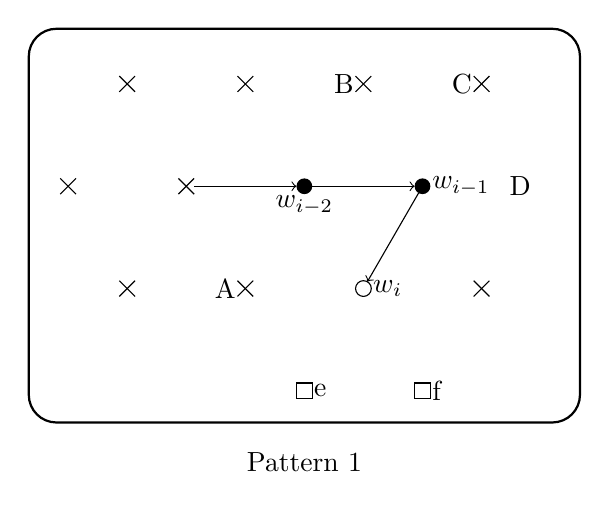
\begin{tikzpicture}
          \draw[thick, rounded corners = 10pt]
          (-2,2)--(5,2)--(5,-3)--(-2,-3)-- cycle;

          \draw[transform canvas={shift=(0:0)}](-0.1,-0.1)--(0.1,0.1);
          \draw[transform canvas={shift=(0:0)}](0.1,-0.1)--(-0.1,0.1);
          
          \foreach \theta in {60,-60,120,-120,180}{
            \draw[transform canvas={shift=(\theta:1.5)}](-0.1,-0.1)--(0.1,0.1);
            \draw[transform canvas={shift=(\theta:1.5)}](0.1,-0.1)--(-0.1,0.1);
          }

          \fill(0:1.5) circle [radius=0.1];
          \draw[->] (0:0.1)--(0:1.4);

          \node[left] at (-60:1.5) {A};

          \begin{scope}[shift=(0:3)]
            \fill(0,0) circle [radius=0.1];

            
            \foreach \theta in {120,60,-60}{
              \draw[transform canvas={shift=(\theta:1.5)}](-0.1,-0.1)--(0.1,0.1);
              \draw[transform canvas={shift=(\theta:1.5)}](0.1,-0.1)--(-0.1,0.1);
            }

            \draw[->] (180:1.4)--(180:0.1);
            \draw[->] (-120:0.1)--(-120:1.4);

            \node[below] at (180:1.5) {$w_{i-2}$};
            \node[right] at (0:0) {$w_{i-1}$};
            \node[right] at (-120:1.5) {$w_i$};

            \node[left] at (120:1.5) {B};
            \node[left] at (60:1.5) {C};
            \node[left] at (0:1.5) {D};

            \begin{scope}[shift=(-120:1.5)]
              \draw(0,0) circle [radius=0.1];
              \foreach \theta in {-120,-60}{
                \draw[transform canvas={shift=(\theta:1.5)}](-0.1,-0.1) rectangle (0.1,0.1);
              }

              \node[right] at (-120:1.5) {e};
              \node[right] at (-60:1.5) {f};
            \end{scope}
            
          \end{scope}

          \node at (1.5,-3.5) {Pattern 1};
        \end{tikzpicture}
      \end{minipage}

      \begin{minipage}{0.48\hsize}
        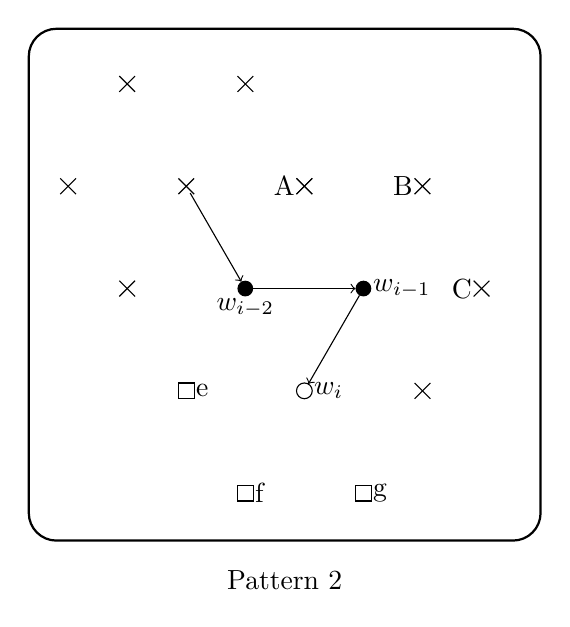
\begin{tikzpicture}
          \draw[thick, rounded corners = 10pt]
          (-2,2)--(4.5,2)--(4.5,-4.5)--(-2,-4.5)-- cycle;

          \draw[transform canvas={shift=(0:0)}](-0.1,-0.1)--(0.1,0.1);
          \draw[transform canvas={shift=(0:0)}](0.1,-0.1)--(-0.1,0.1);
          
          \foreach \theta in {60,0,120,-120,180}{
            \draw[transform canvas={shift=(\theta:1.5)}](-0.1,-0.1)--(0.1,0.1);
            \draw[transform canvas={shift=(\theta:1.5)}](0.1,-0.1)--(-0.1,0.1);
          }

          \draw[->] (-60:0.1)--(-60:1.4);


          \begin{scope}[shift=(-60:1.5),shift=(0:1.5)]
            \fill(0,0) circle [radius=0.1];
            \fill(180:1.5) circle [radius=0.1];

            
            \foreach \theta in {120,60,0,-60}{
              \draw[transform canvas={shift=(\theta:1.5)}](-0.1,-0.1)--(0.1,0.1);
              \draw[transform canvas={shift=(\theta:1.5)}](0.1,-0.1)--(-0.1,0.1);
            }

            \draw[->] (180:1.4)--(180:0.1);
            \draw[->] (-120:0.1)--(-120:1.4);

            \node[below] at (180:1.5) {$w_{i-2}$};
            \node[right] at (0:0) {$w_{i-1}$};
            \node[right] at (-120:1.5) {$w_i$};

            \node[left] at (120:1.5) {A};
            \node[left] at (60:1.5) {B};
            \node[left] at (0:1.5) {C};

            \begin{scope}[shift=(-120:1.5)]
              \draw(0,0) circle [radius=0.1];
              \foreach \theta in {180,-120,-60}{
                \draw[transform canvas={shift=(\theta:1.5)}](-0.1,-0.1) rectangle (0.1,0.1);
              }

              \node[right] at (180:1.5) {e};
              \node[right] at (-120:1.5) {f};
              \node[right] at (-60:1.5) {g};
            \end{scope}
            
          \end{scope}

          \node at (1.25,-5) {Pattern 2};
        \end{tikzpicture}
      \end{minipage}

      
      
    \end{tabular}
    \caption{Case of $S[i-2..i] = tbt$}
    \label{TTT_tunnelC_enter_usingTunnel}
  \end{center}
\end{figure}


\subsubsection{Case of $S[i-2..i] = bbt$}
Let us consider number of consumed by $w_{i-2}$ (Fig.\ref{TTT_tunnelC_enter_usingBond}).

\begin{itemize}
\item{$w_{i-2}$ consumes one binding}\\
  In this situation, $w_{i-2}$ supplies one active binding whereas $w_{i}$ consumes this binding. In addtion, $w_{i-1}$ has to bound to one of A, B, C.
  Thus, in this cases consume some binding capabilities.

\item{$w_{i-2}$ consumes two bindings}\\
  In this case, $w_{i-2}$ already consumes two binding. $w_{i-1}$ has to be bound. $w_i$ supplies at most two bindings. Thus, in this cases consume some binding capabilities.
\end{itemize}



\begin{figure}
  \begin{center}
    \begin{tabular}{cc}
      
      \begin{minipage}{0.48\hsize}
        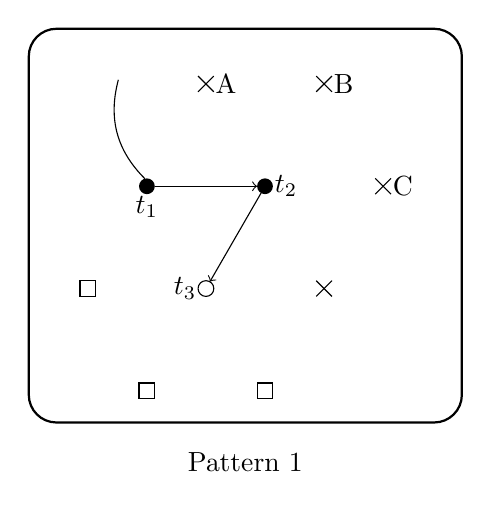
\begin{tikzpicture}
          \draw[thick, rounded corners = 10pt]
          (-3,2)--(2.5,2)--(2.5,-3)--(-3,-3)-- cycle;
          
          \foreach \theta in {60,-60,120,0}{
            \draw[transform canvas={shift=(\theta:1.5)}](-0.1,-0.1)--(0.1,0.1);
            \draw[transform canvas={shift=(\theta:1.5)}](0.1,-0.1)--(-0.1,0.1);
          }

          \fill(180:1.5) circle [radius=0.1];
          \fill(0:0) circle [radius=0.1];

          \draw[transform canvas={shift=(180:1.5)}] (105:1.4) edge[bend right] (105:0.1);
          \draw[->] (180:1.4) -- (180:0.1);
          \draw[->] (-120:0.1) -- (-120:1.4);

          \node[below] at (180:1.5) {$t_1$};
          \node[right] at (0:0) {$t_2$};
          \node[left] at (-120:1.5) {$t_3$};

          \node[right] at (120:1.5) {A};
          \node[right] at (60:1.5) {B};
          \node[right] at (0:1.5) {C};

          \begin{scope}[shift=(-120:1.5)]
            \draw(0,0) circle [radius=0.1];
            \foreach \theta in {-120,-60,180}{
              \draw[transform canvas={shift=(\theta:1.5)}](-0.1,-0.1) rectangle (0.1,0.1);
            }
            
          \end{scope}
          
          \node at (-0.25,-3.5) {Pattern 1};
        \end{tikzpicture}
      \end{minipage}

      
      
    \end{tabular}
    \caption{Case of $S[i-2..i] = bbt$}
    \label{TTT_tunnelC_enter_usingBond}
  \end{center}
\end{figure}


By Tunnel Troll Theorem, any tunnel sections which represented in $bbt^+$ or $bt^+bt^+$ consume binding capabilities. If the sequence $S$ is free from any subsequence of the form $bt^+bt^+$, then it can factorize as $S = u_1 u_2 u_3 \cdots$ for some $u_1 , u_2 , u_3 , \cdots \in \{b\} \cup bbt^+$. Assume the length of $\sigma$ is $n$, seed supplies at most $2n$ binding capabilities. Therefore formula \ref{TTT_only_hold} hold.

\begin{eqnarray}
  \exists i \in \mathbb{N} \quad s.t. \quad u_{i-1} , u_i , u_{i+1} , u_{i+2} , \cdots \in \{ b \}
  \label{TTT_only_bond}
\end{eqnarray}


Let us represent $S$ as $S[i.i+1...] = v_i v_{i+1} v_{i+2} \cdots$ for some $v_i, v_{i+1}, v_{i+2}, \cdots \in \{ a, o\}$ where if $v_k$ is $a$, then $v_{k+1}$ is bound to $v_{k-1}$, if $v_k$ is $o$, then $v_{k+1}$ is NOT bound to $v_{k-1}$.


Let us consider the case of $v_k$ is $o$. See Fig.\ref{TTT_case_of_o}. $v_{i-1}$ consumes some binding capabilities because $S[i-1]$ is $b$. If the number of $v_{i-1}$'s bindings is one binding, then $v_{i+1}$ has to be bound except A or B so that $v_{i+1}$ must consumes two bindings except the case of A and B are occupied and $v_i$ consumes at least one binding. If A and B are occupied, then $v_{i-1}$'s binginds are inactive that is $v_{i-1}$ consumes two binding capabilities. Therefore, this case consumes binding capabilities. If $v_{i-1}$ dose Not have any bindings, then $v_{i-1}$ already consumes two bindings. In addition, $v_i$ and $v_{i+1}$ consume at least one binding. Therefore this case consumes binding capabilities. Thus, the formula \ref{TTT_only_a} hold and according to the formula \ref{TTT_only_bond} and the formula \ref{TTT_only_a}, the formula \ref{TTT_structure} is hold.

\begin{eqnarray}
  \exists j \in \mathbb{N} \quad s.t. \quad u_j , u_{j+1} , u_{j+2} , \cdots \in \{ a \}
  \label{TTT_only_a}
\end{eqnarray}

\begin{eqnarray}
  | S | > \forall m \in \mathbb{N} \quad \to \quad \exists n \in \mathbb{N} \quad s.t. \quad S[n], S[n+1], \cdots \in \{ a \}
  \label{TTT_structure}
\end{eqnarray}

\begin{figure}
  \begin{center}
    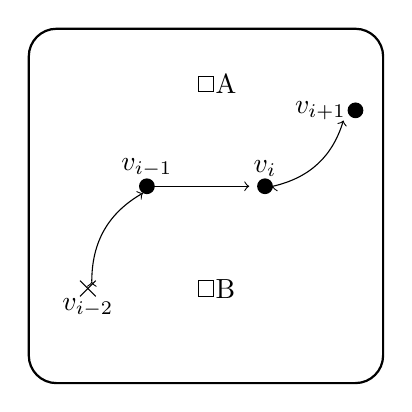
\begin{tikzpicture}
      \draw[thick, rounded corners = 10pt]
      (-1.5,2)--(3,2)--(3,-2.5)--(-1.5,-2.5)-- cycle;
      
      \draw[transform canvas={shift=(-120:1.5)}](-0.1,-0.1)--(0.1,0.1);
      \draw[transform canvas={shift=(-120:1.5)}](0.1,-0.1)--(-0.1,0.1);
      
      \fill(0:0) circle [radius=0.1];
      \fill(0:1.5) circle [radius=0.1];
      \fill[shift=(0:1.5)](40:1.5) circle [radius=0.1];

      
      \draw[->] (-120:1.4) edge[bend left] (-120:0.1);
      \draw[->] (0:0) -- (0:1.3);
      \draw[->,transform canvas={shift=(0:1.5)}] (0:0.1) edge[bend right] (40:1.3);

      \draw [shift=(60:1.5)] (-0.1,-0.1) rectangle (0.1,0.1);
      \draw [shift=(-60:1.5)] (-0.1,-0.1) rectangle (0.1,0.1);
      
      \node[below] at (-120:1.5) {$v_{i-2}$};
      \node[above] at (0:0) {$v_{i-1}$};
      \node[above] at (0:1.5) {$v_i$};
      \node[left, shift=(0:1.5)] at (40:1.5) {$v_{i+1}$};

      \node[right] at (60:1.5) {A};
      \node[right] at (-60:1.5) {B};
        
    \end{tikzpicture}
    \caption{Case of $S[i$}
    \label{TTT_case_of_o}
  \end{center}
\end{figure}

\end{document}
